\chapter[Análisis]{Análisis}

\section*{Procesos de negocio futuros}

Con OnCuidar, el seguimiento domiciliario cambia en tres aspectos. El cuidador
registra los signos y síntomas en la aplicación en lugar de anotarlos en papel,
resuelve sus dudas con contenido validado en la biblioteca o el asistente y
recibe una clasificación del nivel de alerta en cada registro. La
Figura~\ref{fig:bpmn-futuro} modela el nuevo proceso en notación BPMN.

\newgeometry{left=2cm, right=2cm, top=1.5cm, bottom=1.5cm}
\begin{landscape}
\begin{figure}[p]
    \centering
    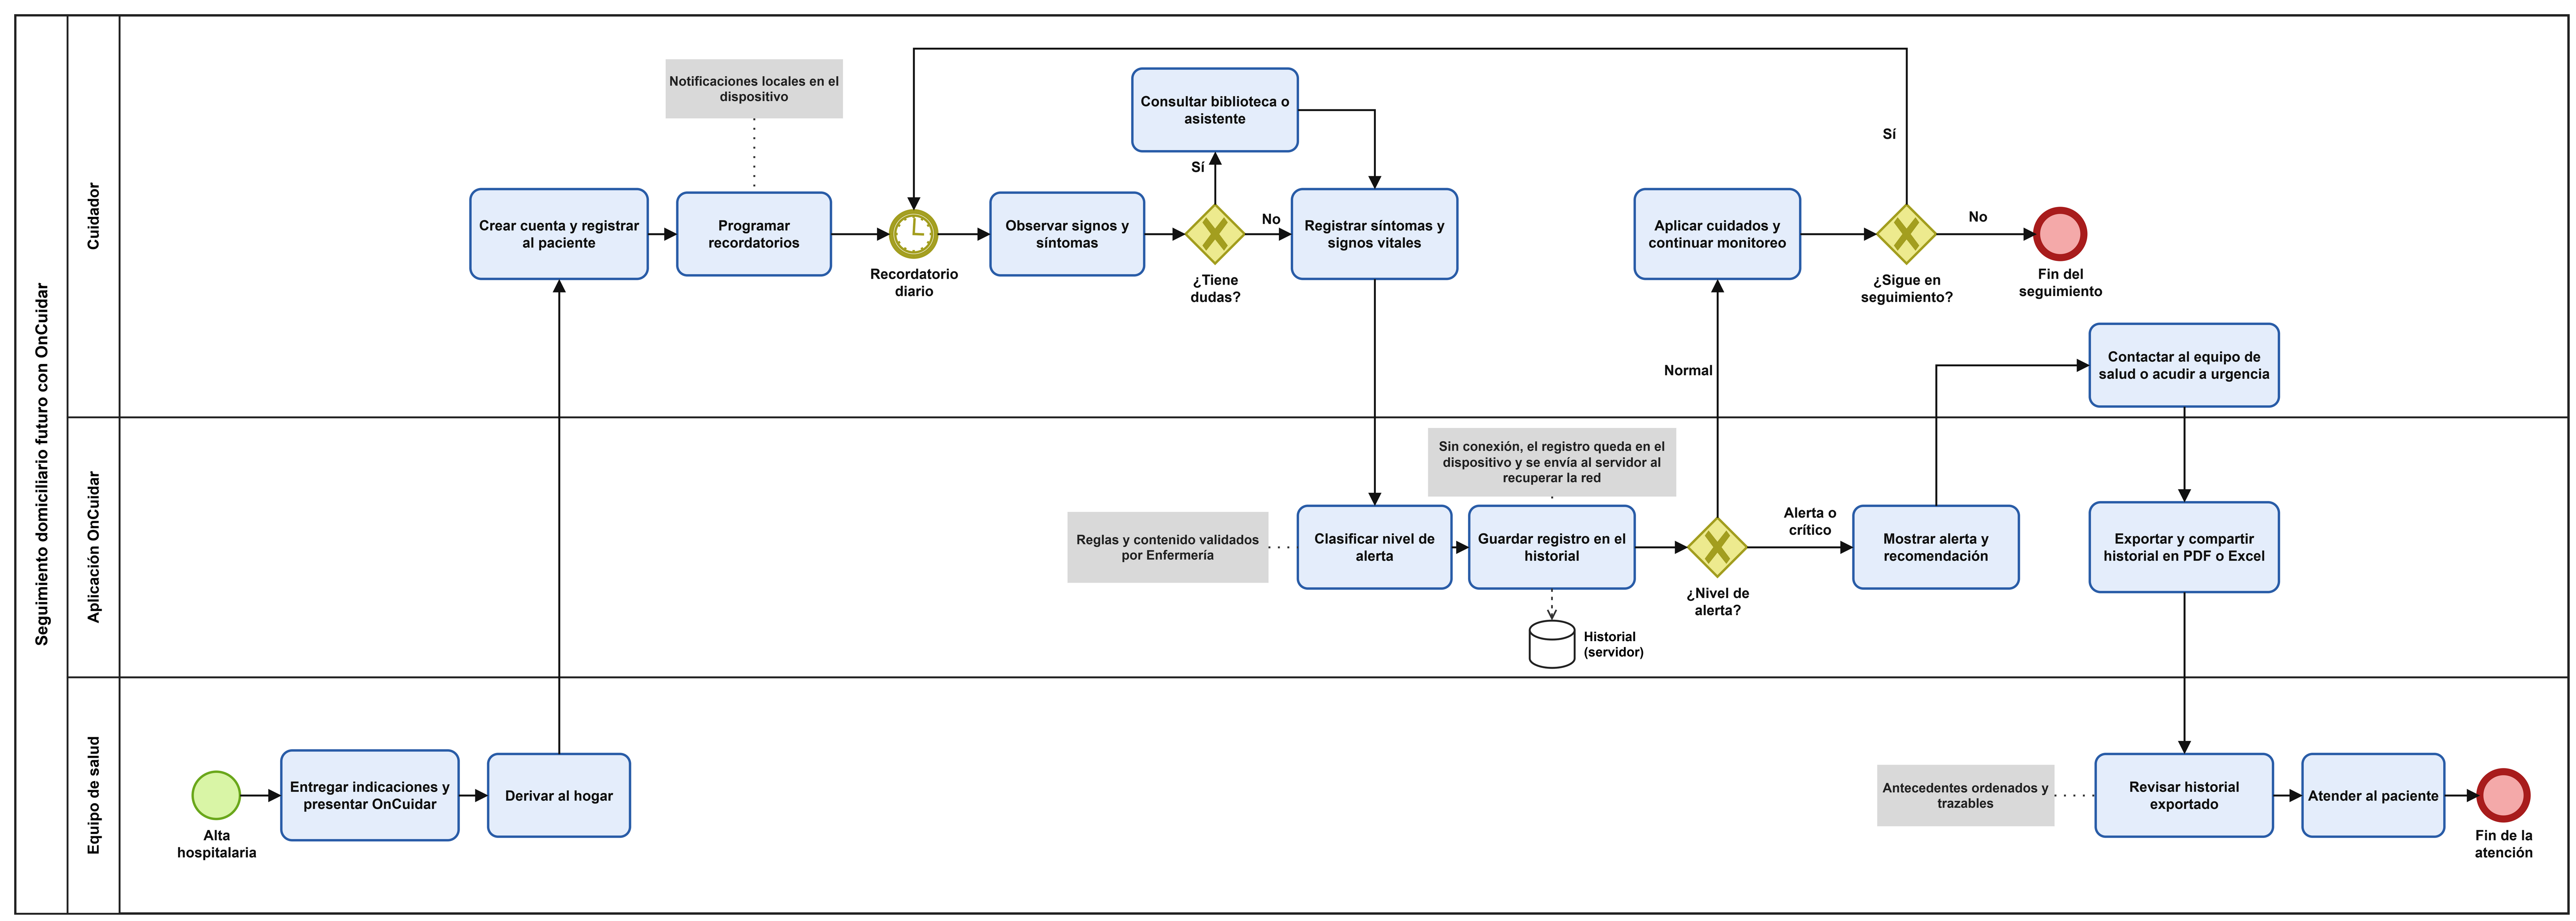
\includegraphics[width=\linewidth, keepaspectratio]{figures/bpmn/bpmn-futuro.png}
    \caption{Proceso de negocio futuro con la aplicación OnCuidar.}
    \label{fig:bpmn-futuro}
\end{figure}
\end{landscape}
\restoregeometry

El proceso comienza con el alta, cuando el equipo de salud entrega las
indicaciones y presenta la aplicación. En el hogar, el cuidador crea su cuenta,
registra al paciente y programa los recordatorios. Cuando suena el recordatorio
diario, observa los signos y síntomas y, si tiene dudas, consulta la biblioteca
o el asistente antes de registrar la valoración. La aplicación clasifica el
nivel de alerta con el motor de reglas y guarda el registro en el historial; sin
conexión, lo conserva en el dispositivo y lo envía al servidor al recuperar la red. Si
el nivel es normal, el cuidador continúa el monitoreo hasta el siguiente
recordatorio. Si es de alerta o crítico, la aplicación muestra la alerta con su
recomendación y el cuidador contacta al equipo de salud o acude a urgencia. En
el control, exporta y comparte el historial en PDF o Excel, y el equipo clínico
revisa antecedentes ordenados en lugar de reconstruirlos desde el relato.

La aplicación no reemplaza la decisión clínica. Su función es acortar el tiempo
entre la aparición de un signo de alerta y el contacto con el equipo de salud, y
mejorar la calidad de la información disponible en cada control.

\section[Diagrama de Flujo de Datos]{Diagrama de flujo de datos}

Según la plantilla, este ítem es excluyente con el diagrama de casos de uso. El
proyecto modela la funcionalidad mediante casos de uso, desarrollados en la
sección siguiente.

\section[Casos de Uso]{Diagrama de casos de uso}

La Figura~\ref{fig:casos-uso} presenta los casos de uso del sistema. Cada
requerimiento funcional del capítulo~4 queda representado por al menos un caso
de uso, como detalla el Anexo de trazabilidad.

\begin{figure}[H]
    \centering
    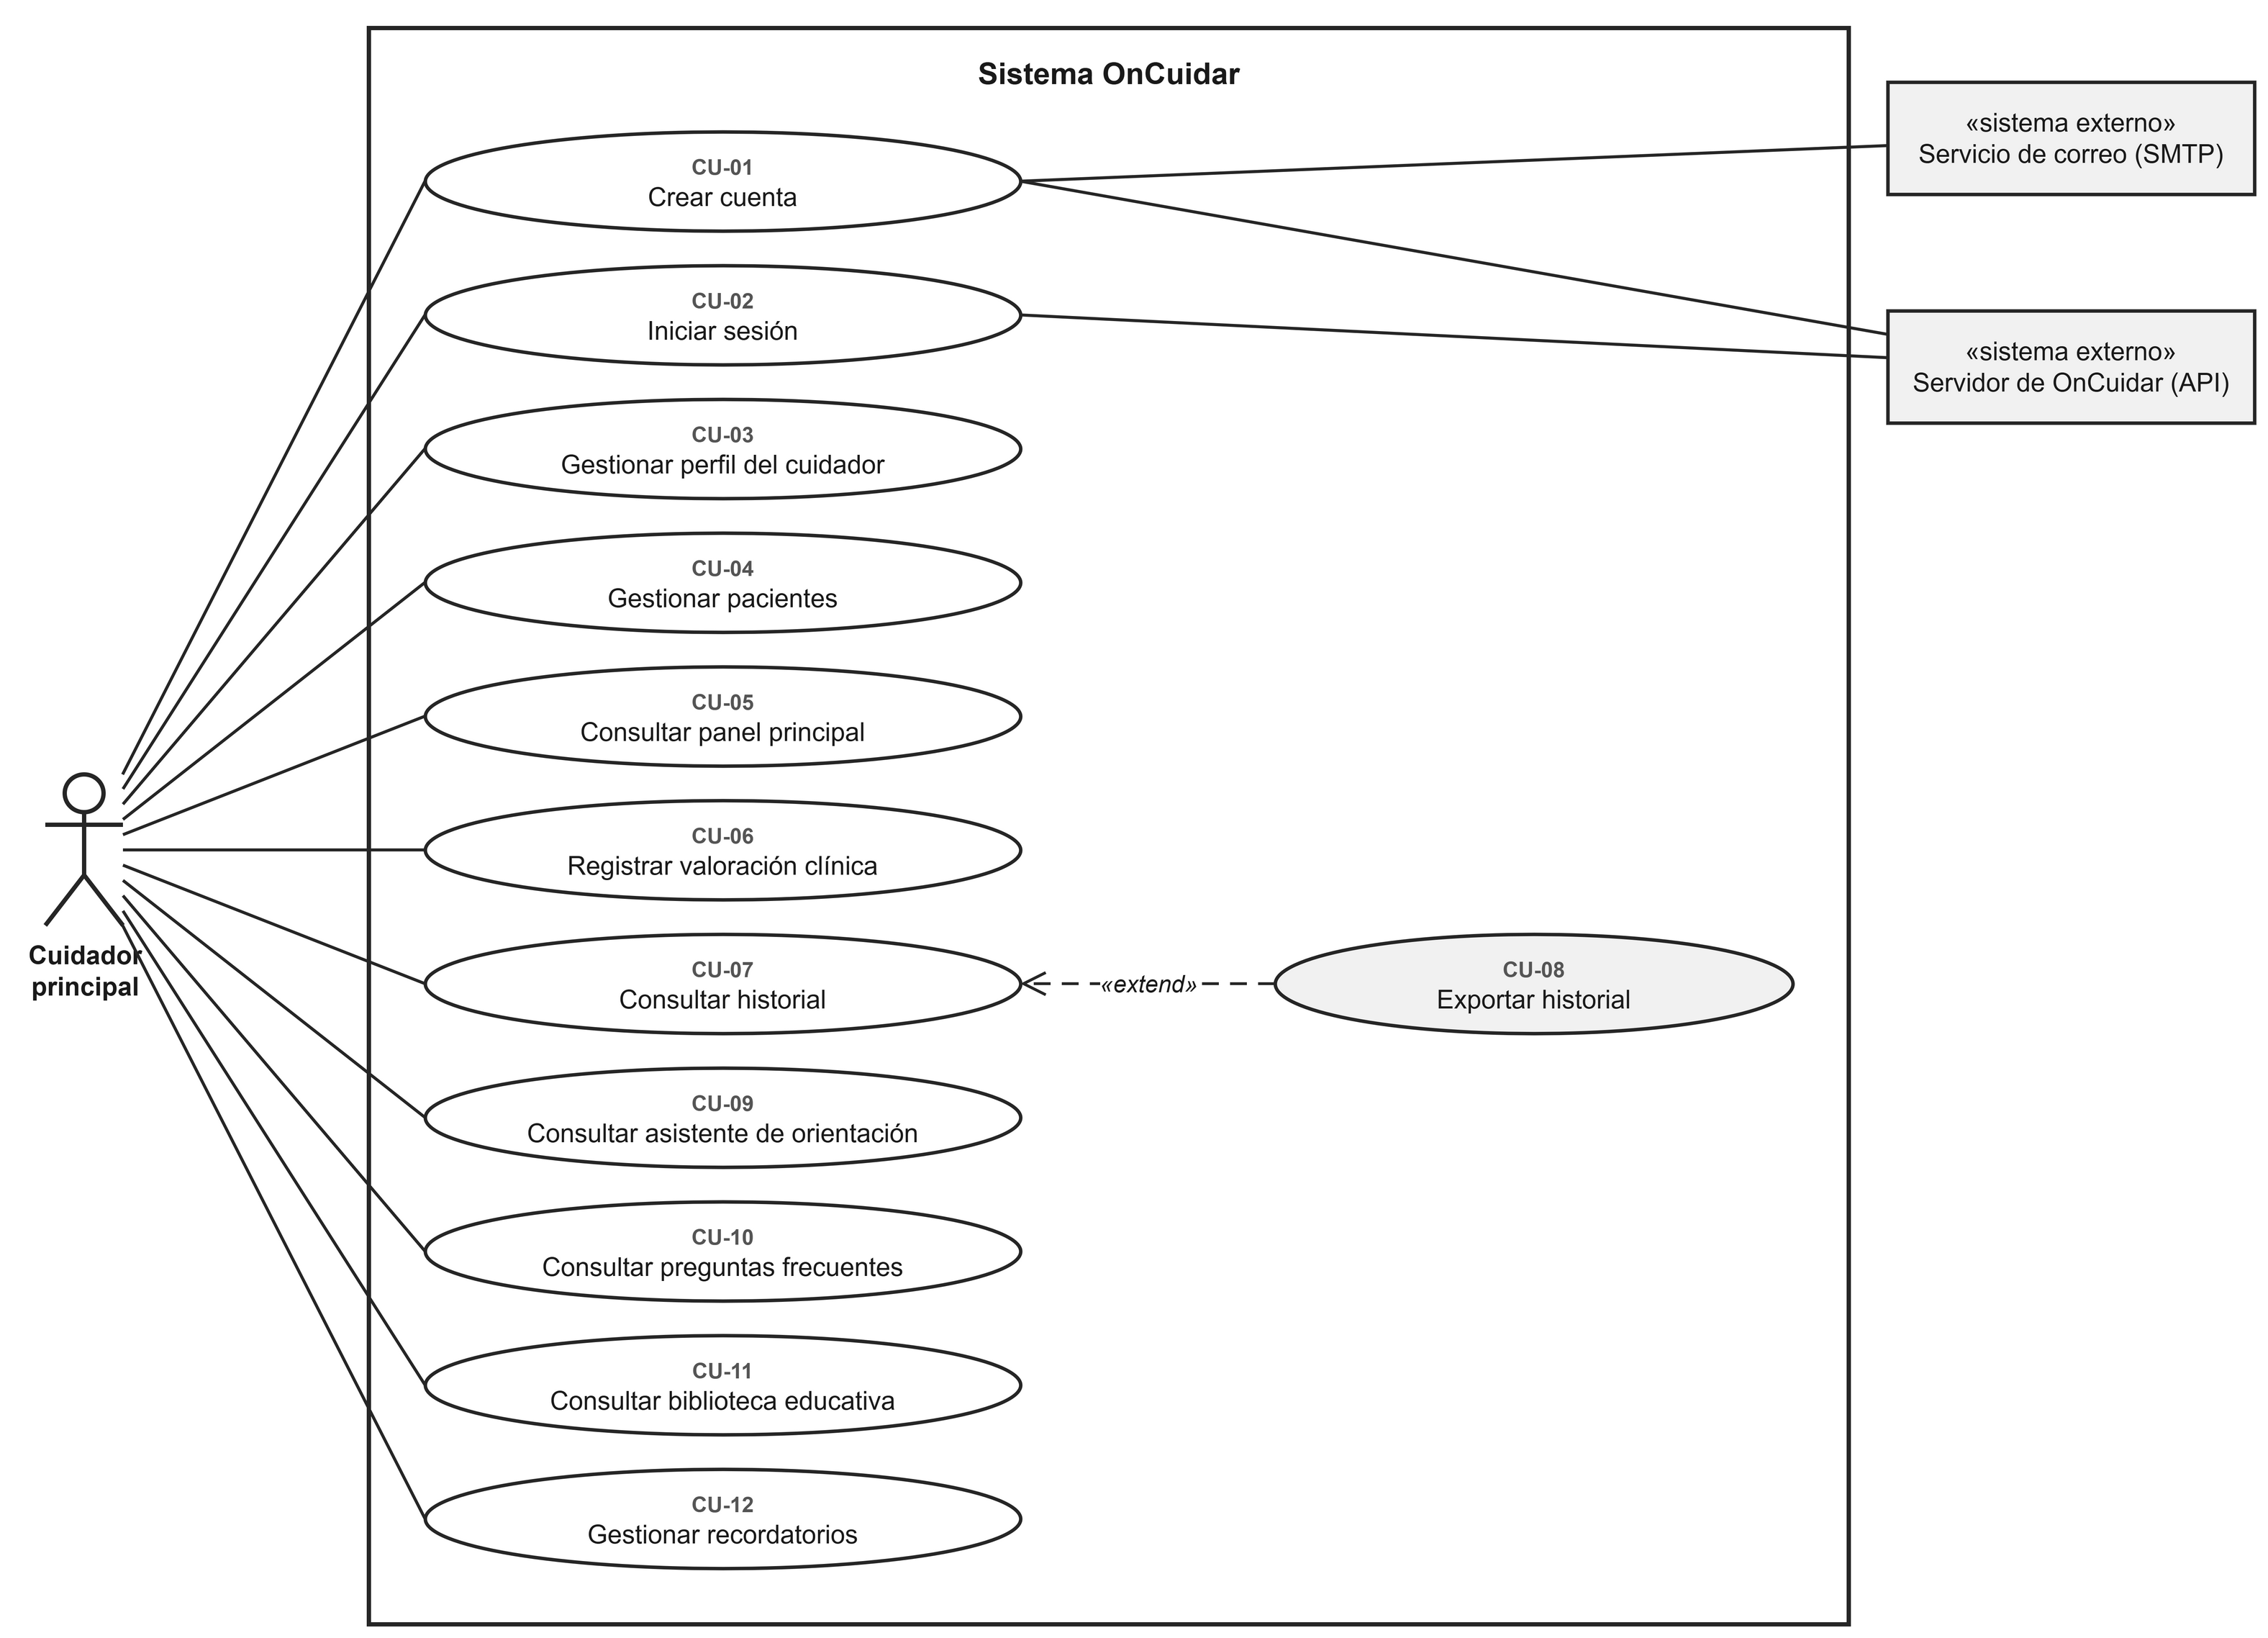
\includegraphics[width=0.92\textwidth, keepaspectratio]{figures/casos-uso/cu-general.png}
    \caption{Diagrama de casos de uso de OnCuidar.}
    \label{fig:casos-uso}
\end{figure}

\subsection[Actores]{Actores}

\begin{table}[H]
\centering
\small
\tablazebra
\caption{Actores del sistema.}
\label{tab:actores}
\begin{tabularx}{\textwidth}{P{0.62}P{1.20}P{0.88}P{1.30}}
\toprule
\filaencabezado \encab{Actor} & \encab{Rol o funciones} & \encab{Conocimientos técnicos} & \encab{Privilegios y funcionalidades} \\
\midrule
Cuidador principal &
Madre, padre o tutor que acompaña al paciente en el hogar, registra su
evolución y aplica las indicaciones del equipo de salud. &
Básicos. Maneja un teléfono inteligente, pero no tiene formación técnica ni
clínica. &
Accede a todas las funciones de la aplicación, limitadas a sus propios datos y a
los de sus pacientes. \\
Servidor de OnCuidar (API) &
Servicio que autentica a los usuarios y almacena los datos de la aplicación en
la base de datos PostgreSQL. Se ejecuta en contenedores, en el servidor de la
Universidad del Bío-Bío. &
No aplica. &
Valida credenciales, entrega al dispositivo la clave de datos del cuidador,
rechaza los datos sensibles en claro y solo permite acceder a los datos del
usuario autenticado. \\
Servicio de correo (SMTP) &
Servicio externo que entrega los correos que envía el servidor. &
No aplica. &
Entrega los enlaces de un solo uso para restablecer la contraseña y confirmar
los correos del cuidador. \\
\bottomrule
\end{tabularx}
\end{table}

\subsection[Diagrama y Descripción]{Casos de uso y descripción}

El cuidador comienza creando una cuenta con sus datos y los de su paciente, y en
los usos siguientes inicia sesión. Desde el perfil puede actualizar sus datos,
agregar otros pacientes y elegir cuál está activo. El panel principal le muestra
el estado del paciente activo y lo lleva a cada módulo.

En su rutina diaria, el cuidador registra la valoración clínica del paciente y
recibe de inmediato su nivel de alerta. Cuando necesita revisar la evolución,
consulta el historial y, antes de un control, lo exporta a PDF o Excel. Si tiene
una duda, puede escribirla al asistente, buscarla en las preguntas frecuentes o
consultar la biblioteca educativa. Para no olvidar tareas, programa
recordatorios. El servidor de OnCuidar participa como
sistema externo en la creación de la cuenta y en el inicio de sesión, y el
servicio de correo, al enviar el enlace que confirma el correo del cuidador o
permite restablecer la contraseña.

\subsection[Especificación de los Casos de Uso]{Especificación de los casos de uso}

Esta sección especifica los cinco casos de uso que concentran el valor del
sistema. Los siete restantes se especifican en el anexo de casos de uso.

\subsubsection{Caso de uso: Registrar valoración clínica}

\begin{figure}[H]
    \centering
    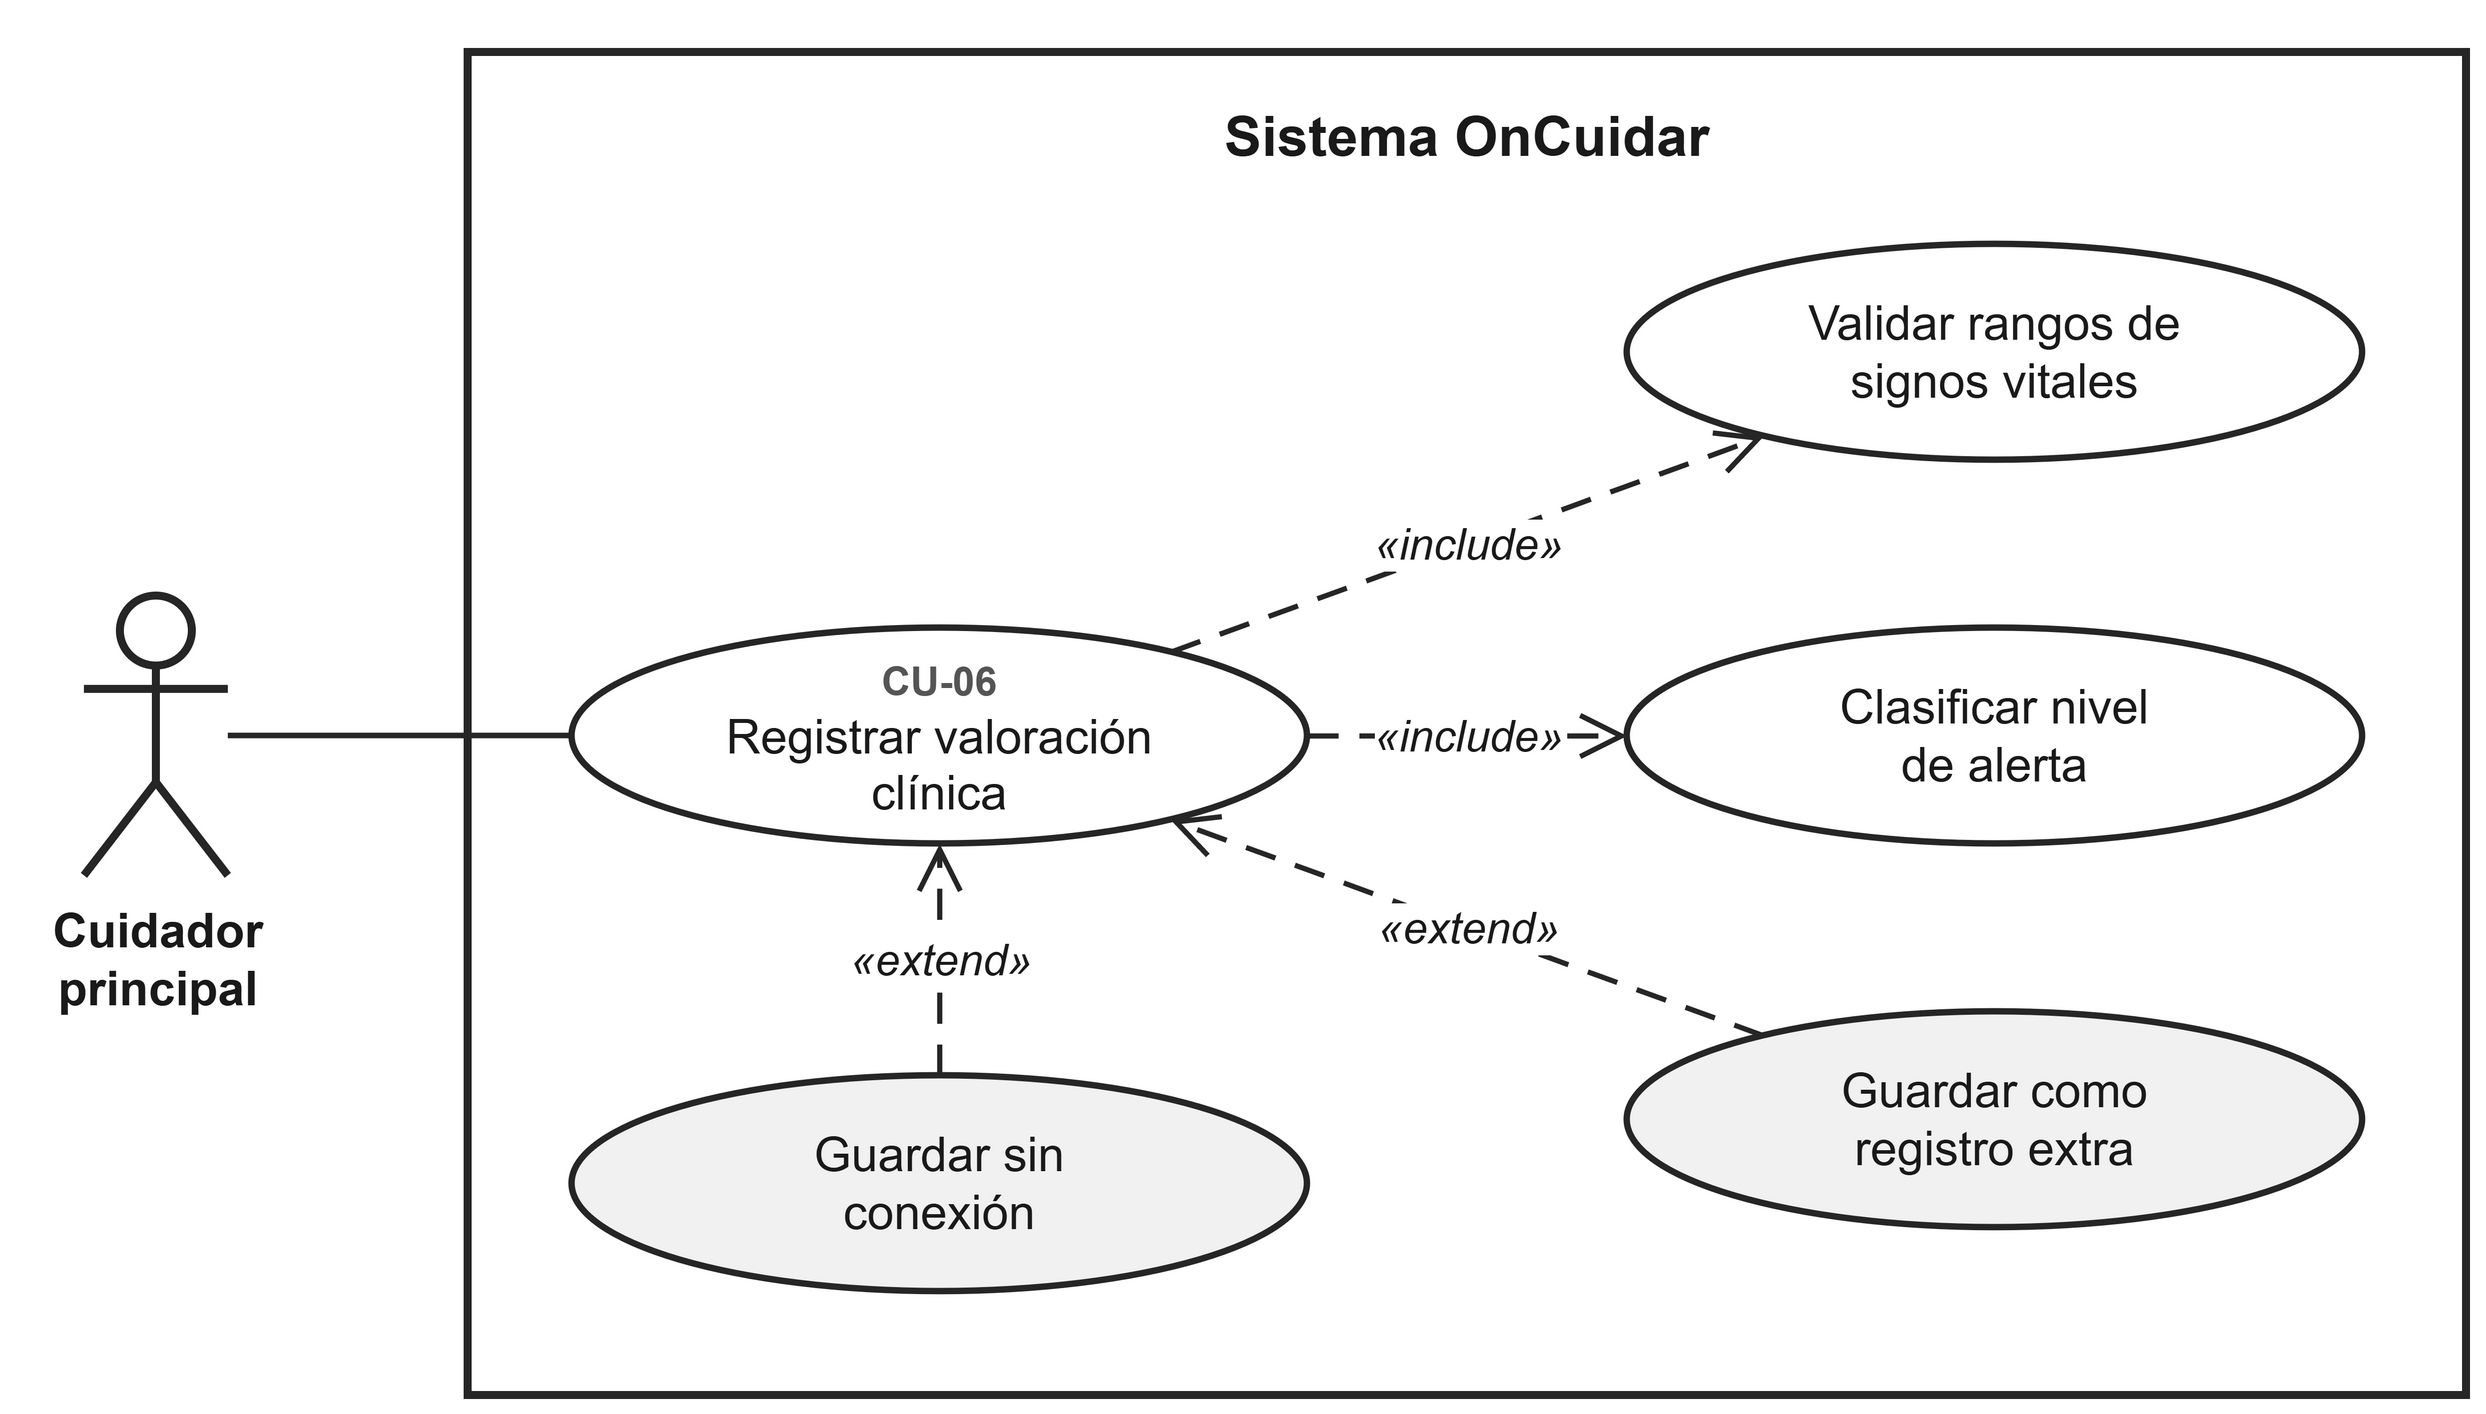
\includegraphics[width=0.9\textwidth, keepaspectratio]{figures/casos-uso/cu-06-registrar-valoracion.png}
    \caption{Diagrama del caso de uso CU-06: registrar valoración clínica.}
    \label{fig:cu-06}
\end{figure}

\begin{table}[H]
\centering
\caption{Especificación del caso de uso CU-06.}
\label{tab:cu-06}
\begin{especificacioncu}{CU-06}{Registrar valoración clínica}
    \cufila{Descripción}{El cuidador registra los signos vitales, los síntomas y
    las observaciones del paciente activo, y el sistema clasifica el nivel de
    alerta del registro.}
    \cufila{Actor}{Cuidador principal.}
    \cufila{Requerimientos}{RF-11, RF-12, RF-13, RF-28.}
    \cufila{Precondiciones}{El cuidador inició sesión y tiene un paciente
    activo.}
    \cuflujo{Flujo de eventos básico}
    \cupaso{1. Selecciona Registro en la barra inferior.}
           {2. Muestra el formulario con el tipo de registro, los signos
           vitales, los síntomas ESAS y las observaciones.}
    \cupaso{3. Ingresa los signos vitales que conoce, la intensidad de cada
           síntoma y, si lo desea, observaciones.}
           {4. Valida que cada signo esté dentro de su rango físico y muestra
           el nivel de alerta calculado.}
    \cupaso{5. Presiona Guardar.}
           {6. Cifra los datos sensibles, guarda el registro con fecha y hora y
           confirma el guardado.}
    \cupaso{}{7. Muestra el nivel de alerta, los motivos detectados y la
           recomendación correspondiente.}
    \cufinflujo
    \cuflujo{Flujos alternativos}
    \cupaso{}{4a. Si un signo está fuera de rango, indica el rango permitido y
           no permite guardar hasta que se corrija.}
    \cupaso{}{6a. Si el paciente alcanzó su tope diario de registros
           programados, guarda el registro como extra.}
    \cupaso{}{6b. Si no hay conexión, guarda el registro en el dispositivo y lo
           lo envía al servidor al recuperar la red.}
    \cufinflujo
    \cufila{Postcondiciones}{El registro queda en el historial del paciente con
    su nivel de alerta y el panel principal se actualiza.}
\end{especificacioncu}
\end{table}

\subsubsection{Caso de uso: Exportar historial}

\begin{figure}[H]
    \centering
    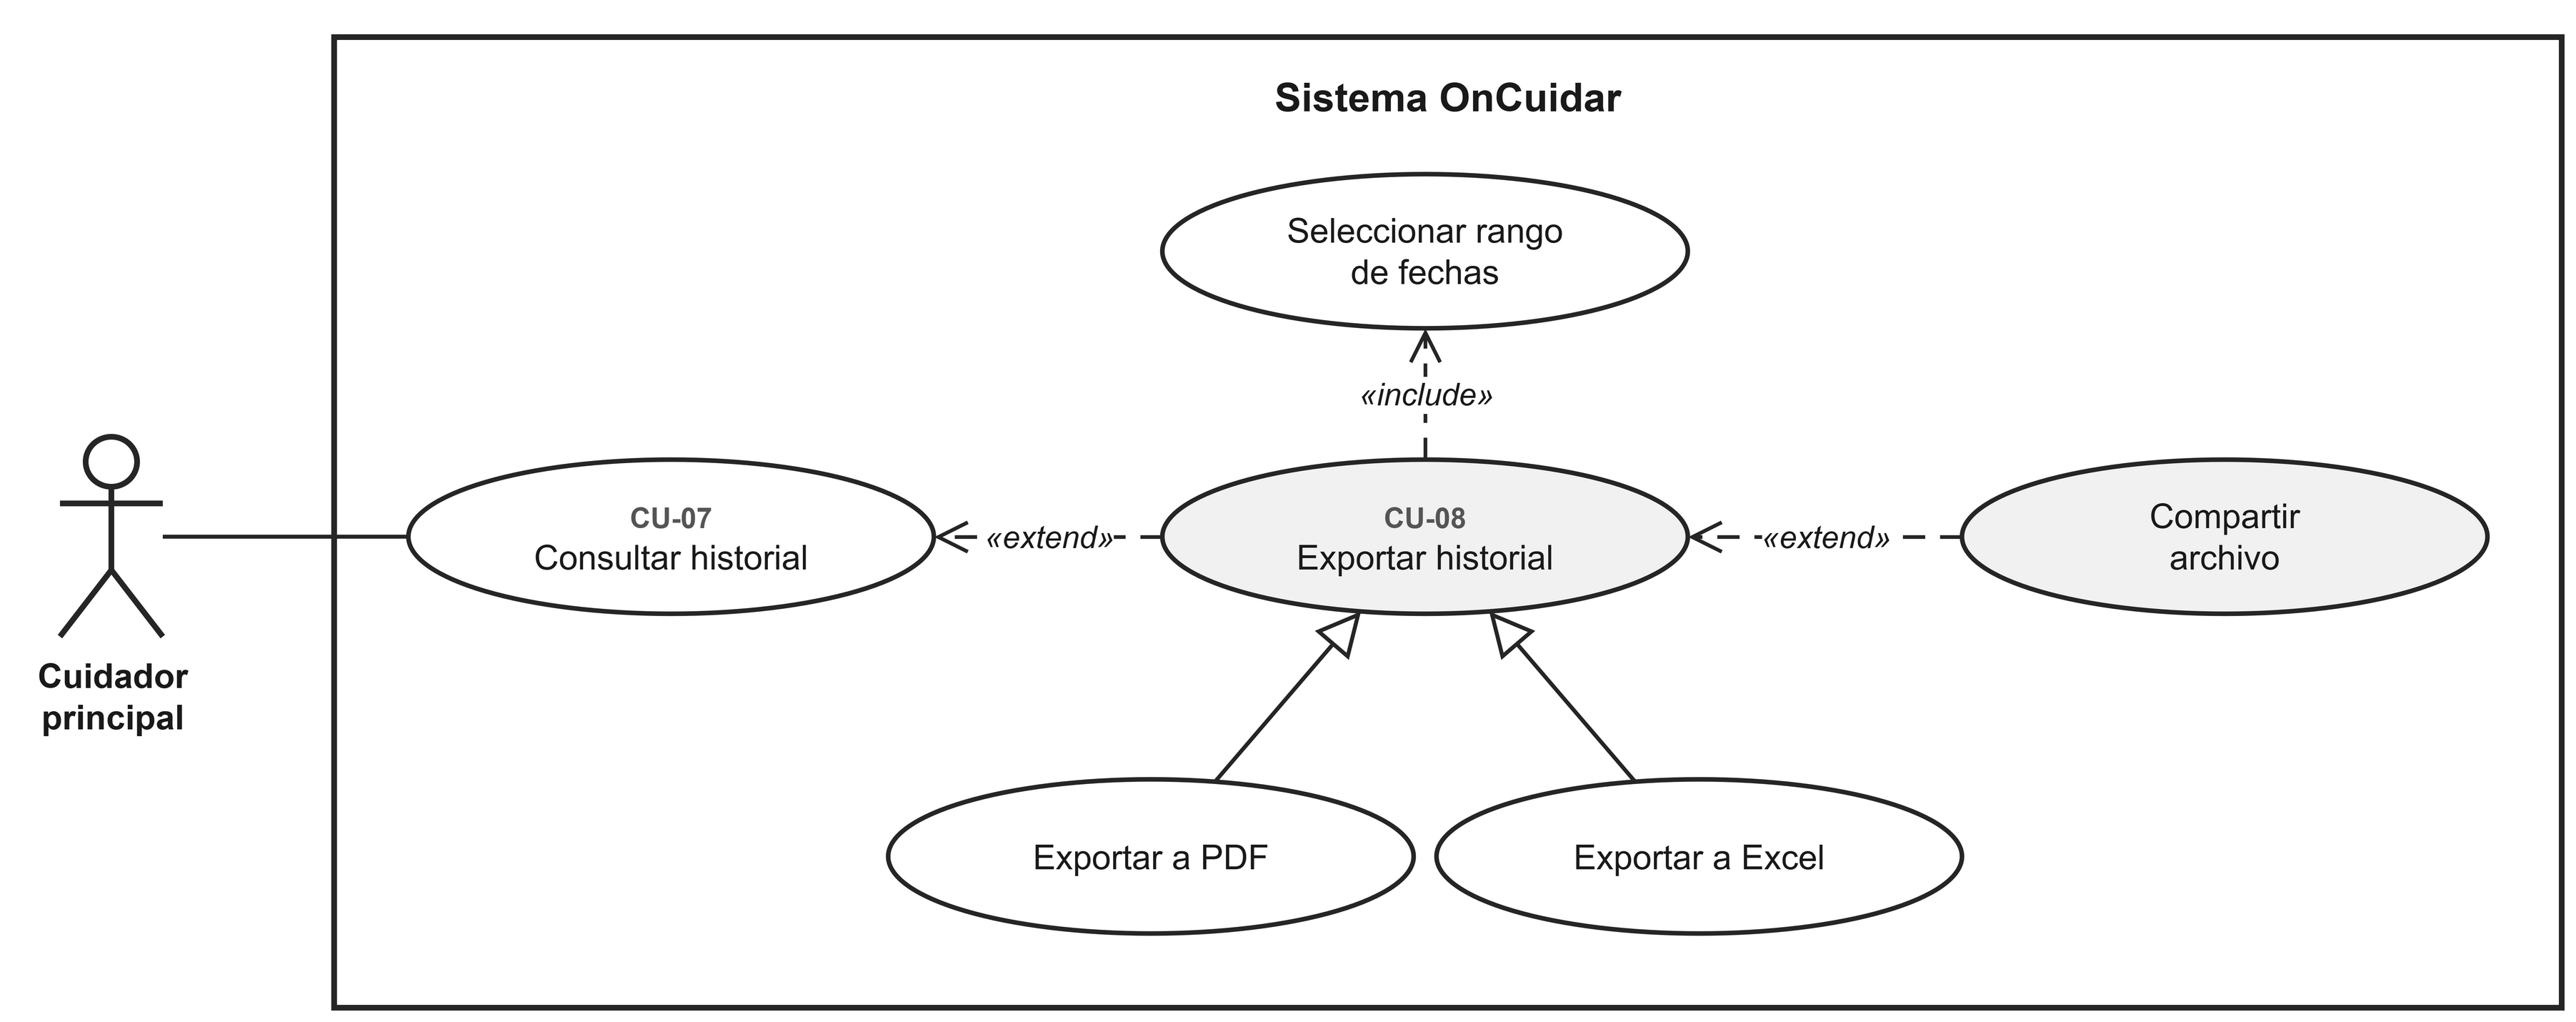
\includegraphics[width=0.9\textwidth, keepaspectratio]{figures/casos-uso/cu-08-exportar-historial.png}
    \caption{Diagrama del caso de uso CU-08: exportar historial.}
    \label{fig:cu-08}
\end{figure}

\begin{table}[H]
\centering
\caption{Especificación del caso de uso CU-08.}
\label{tab:cu-08}
\begin{especificacioncu}{CU-08}{Exportar historial}
    \cufila{Descripción}{El cuidador genera un informe del historial del paciente
    activo en PDF o Excel para presentarlo en un control clínico.}
    \cufila{Actor}{Cuidador principal.}
    \cufila{Requerimientos}{RF-16, RF-17.}
    \cufila{Precondiciones}{El paciente activo tiene registros en el historial.}
    \cuflujo{Flujo de eventos básico}
    \cupaso{1. Desde el historial, elige exportar y selecciona PDF o Excel.}
           {2. Solicita el rango de fechas del informe.}
    \cupaso{3. Indica el rango de fechas.}
           {4. Descifra los registros del rango y genera el archivo con los
           datos del paciente, del cuidador, del centro de salud y del contacto
           de emergencia, junto con el detalle de cada registro.}
    \cupaso{}{5. Guarda el archivo en el dispositivo y ofrece abrirlo o
           compartirlo.}
    \cupaso{6. Abre el archivo o lo comparte.}{}
    \cufinflujo
    \cuflujo{Flujos alternativos}
    \cupaso{}{4a. Si no hay registros en el rango elegido, informa que no hay
           datos para exportar.}
    \cufinflujo
    \cufila{Postcondiciones}{El informe queda guardado en el dispositivo del
    cuidador.}
\end{especificacioncu}
\end{table}

\subsubsection{Caso de uso: Consultar asistente de orientación}

\begin{figure}[H]
    \centering
    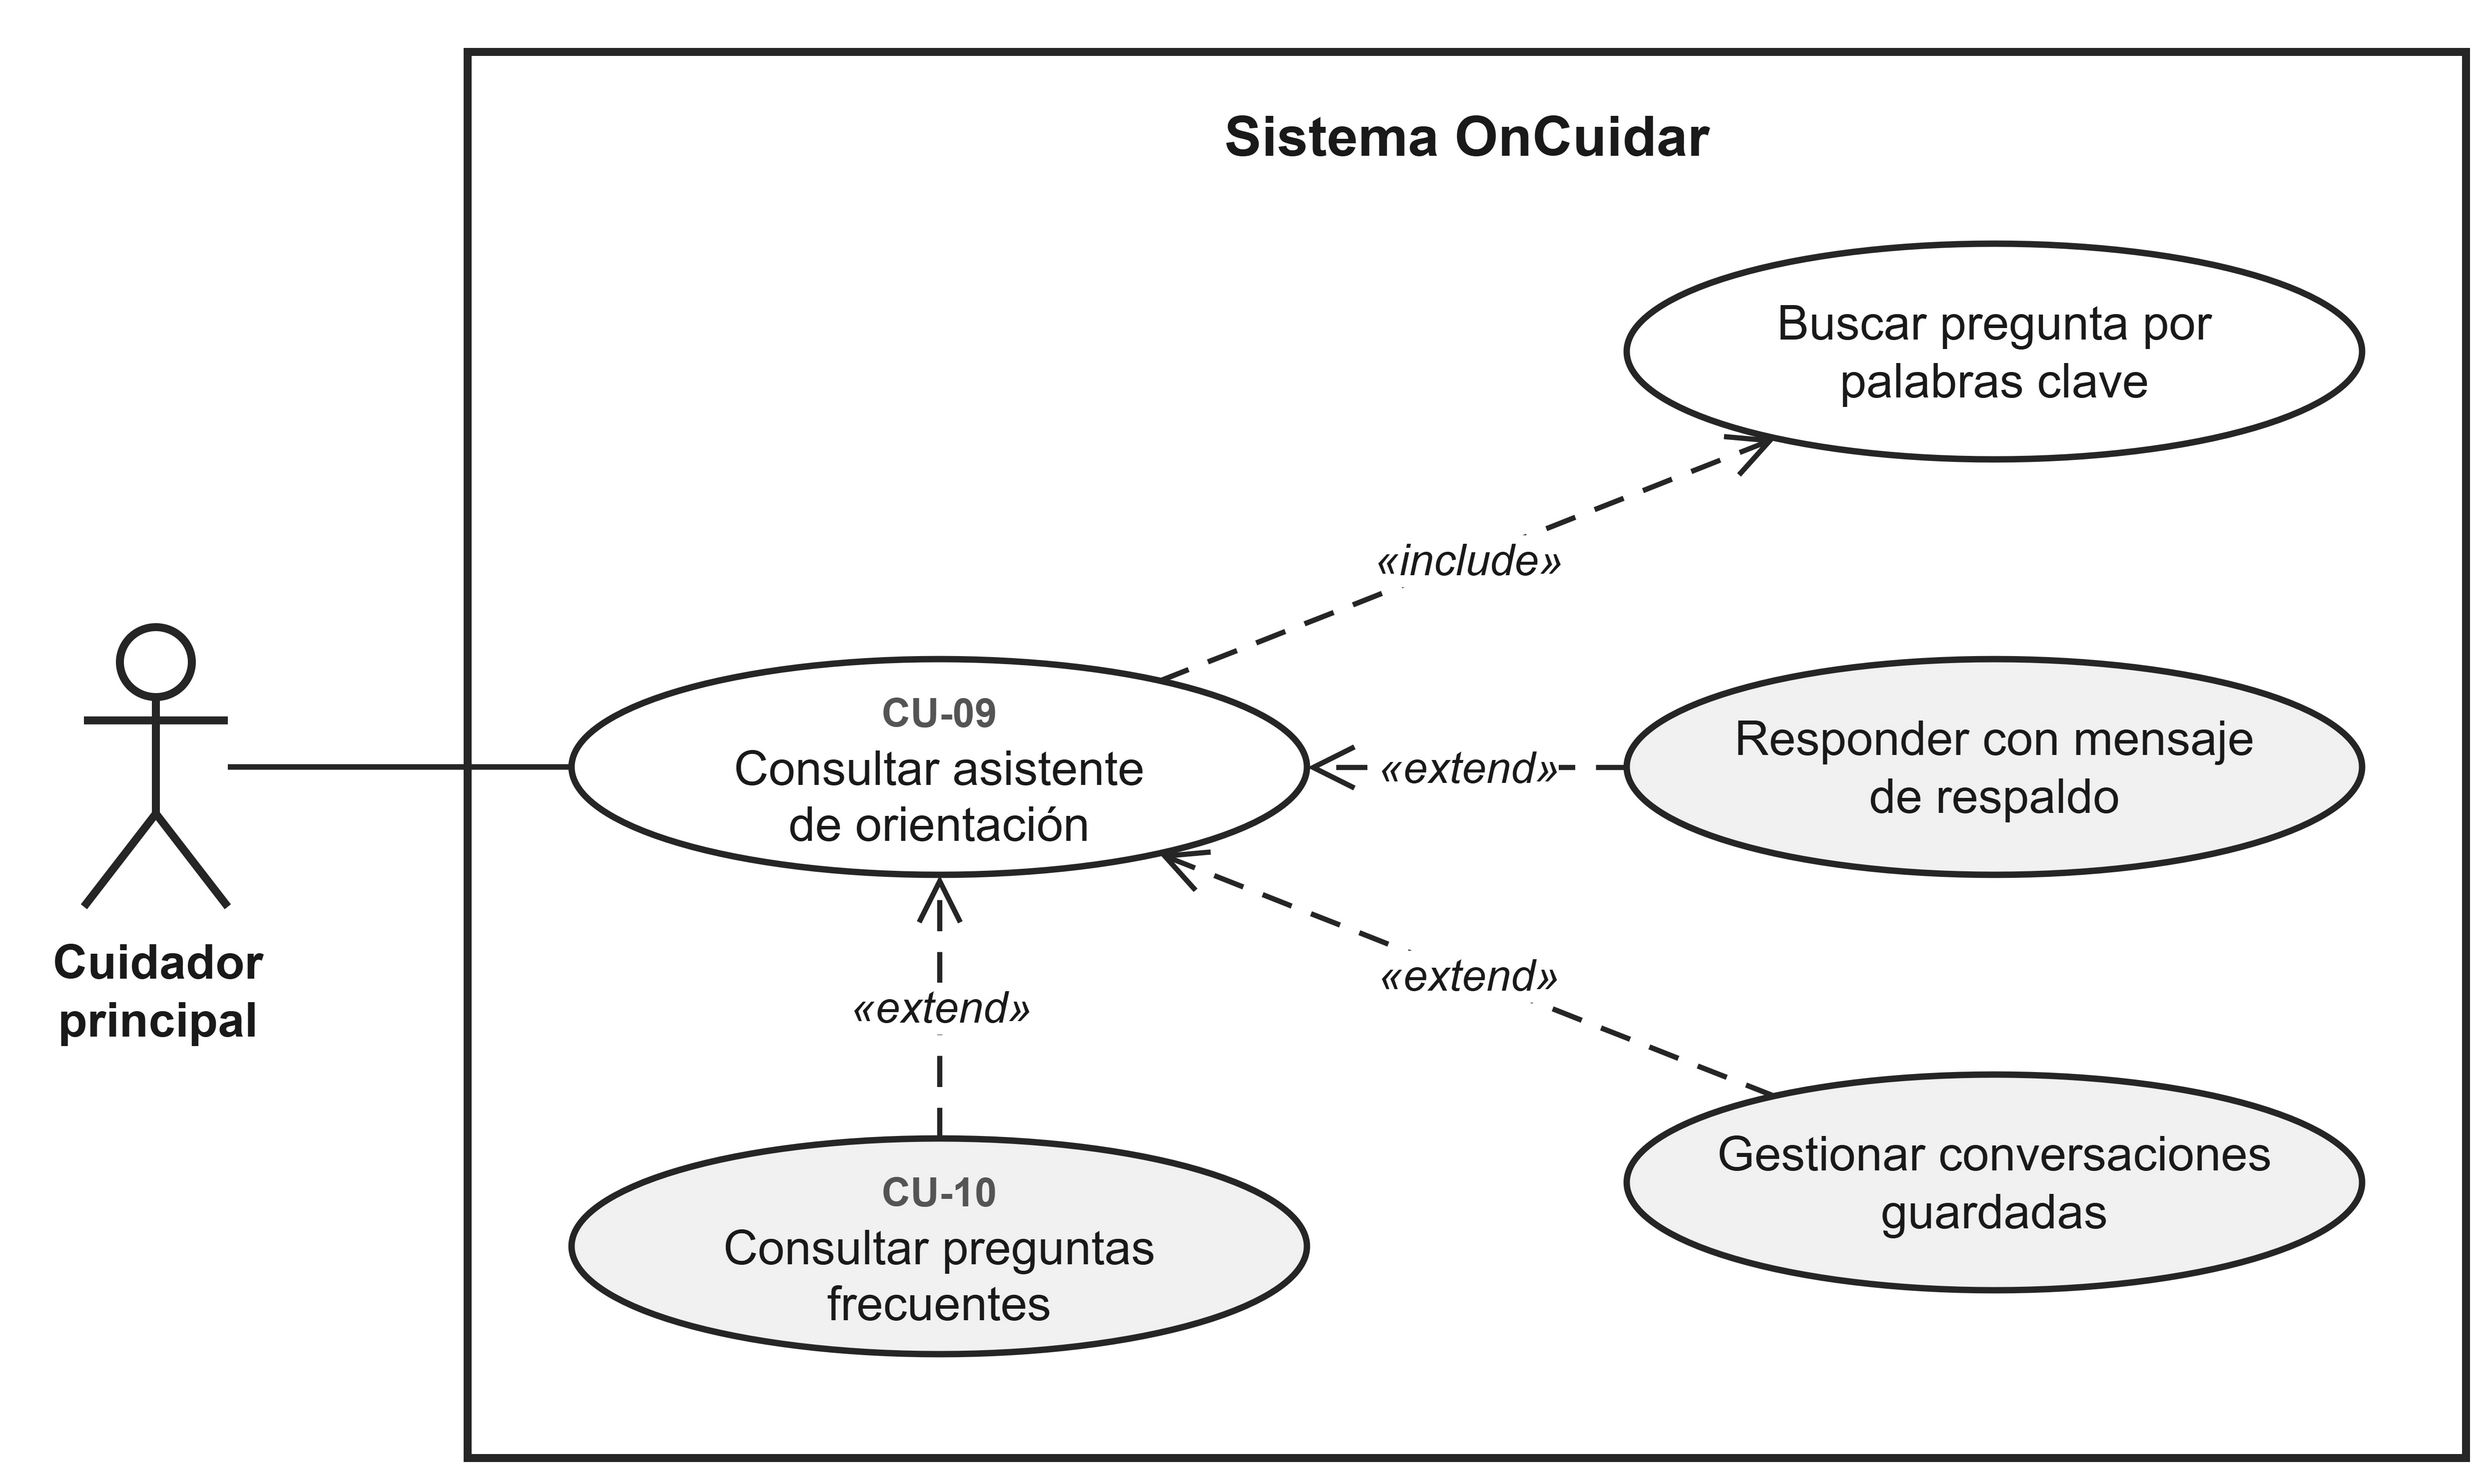
\includegraphics[width=0.9\textwidth, keepaspectratio]{figures/casos-uso/cu-09-asistente.png}
    \caption{Diagrama del caso de uso CU-09: consultar asistente de orientación.}
    \label{fig:cu-09}
\end{figure}

\begin{table}[H]
\centering
\caption{Especificación del caso de uso CU-09.}
\label{tab:cu-09}
\begin{especificacioncu}{CU-09}{Consultar asistente de orientación}
    \cufila{Descripción}{El cuidador escribe una duda y recibe la respuesta de la
    pregunta frecuente validada que mejor coincide con ella.}
    \cufila{Actor}{Cuidador principal.}
    \cufila{Requerimientos}{RF-19, RF-20.}
    \cufila{Precondiciones}{El cuidador inició sesión.}
    \cuflujo{Flujo de eventos básico}
    \cupaso{1. Selecciona Chat en la barra inferior.}
           {2. Muestra un mensaje de bienvenida y preguntas sugeridas.}
    \cupaso{3. Escribe su consulta o elige una pregunta sugerida.}
           {4. Busca la pregunta frecuente que comparte más palabras clave con
           la consulta.}
    \cupaso{}{5. Muestra la respuesta validada y guarda la conversación con un
           título automático.}
    \cupaso{6. Continúa la conversación o sale del chat.}{}
    \cufinflujo
    \cuflujo{Flujos alternativos}
    \cupaso{}{4a. Si ninguna pregunta alcanza la coincidencia mínima, responde
           que aún no tiene una respuesta exacta, sugiere los temas disponibles y
           recomienda consultar al equipo médico.}
    \cupaso{1a. Abre sus conversaciones guardadas.}
           {1b. Las lista por última actividad y permite continuarlas,
           renombrarlas o eliminarlas.}
    \cufinflujo
    \cufila{Postcondiciones}{La conversación queda guardada en la cuenta del
    cuidador, con sus mensajes cifrados.}
\end{especificacioncu}
\end{table}

\subsubsection{Caso de uso: Consultar biblioteca educativa}

\begin{figure}[H]
    \centering
    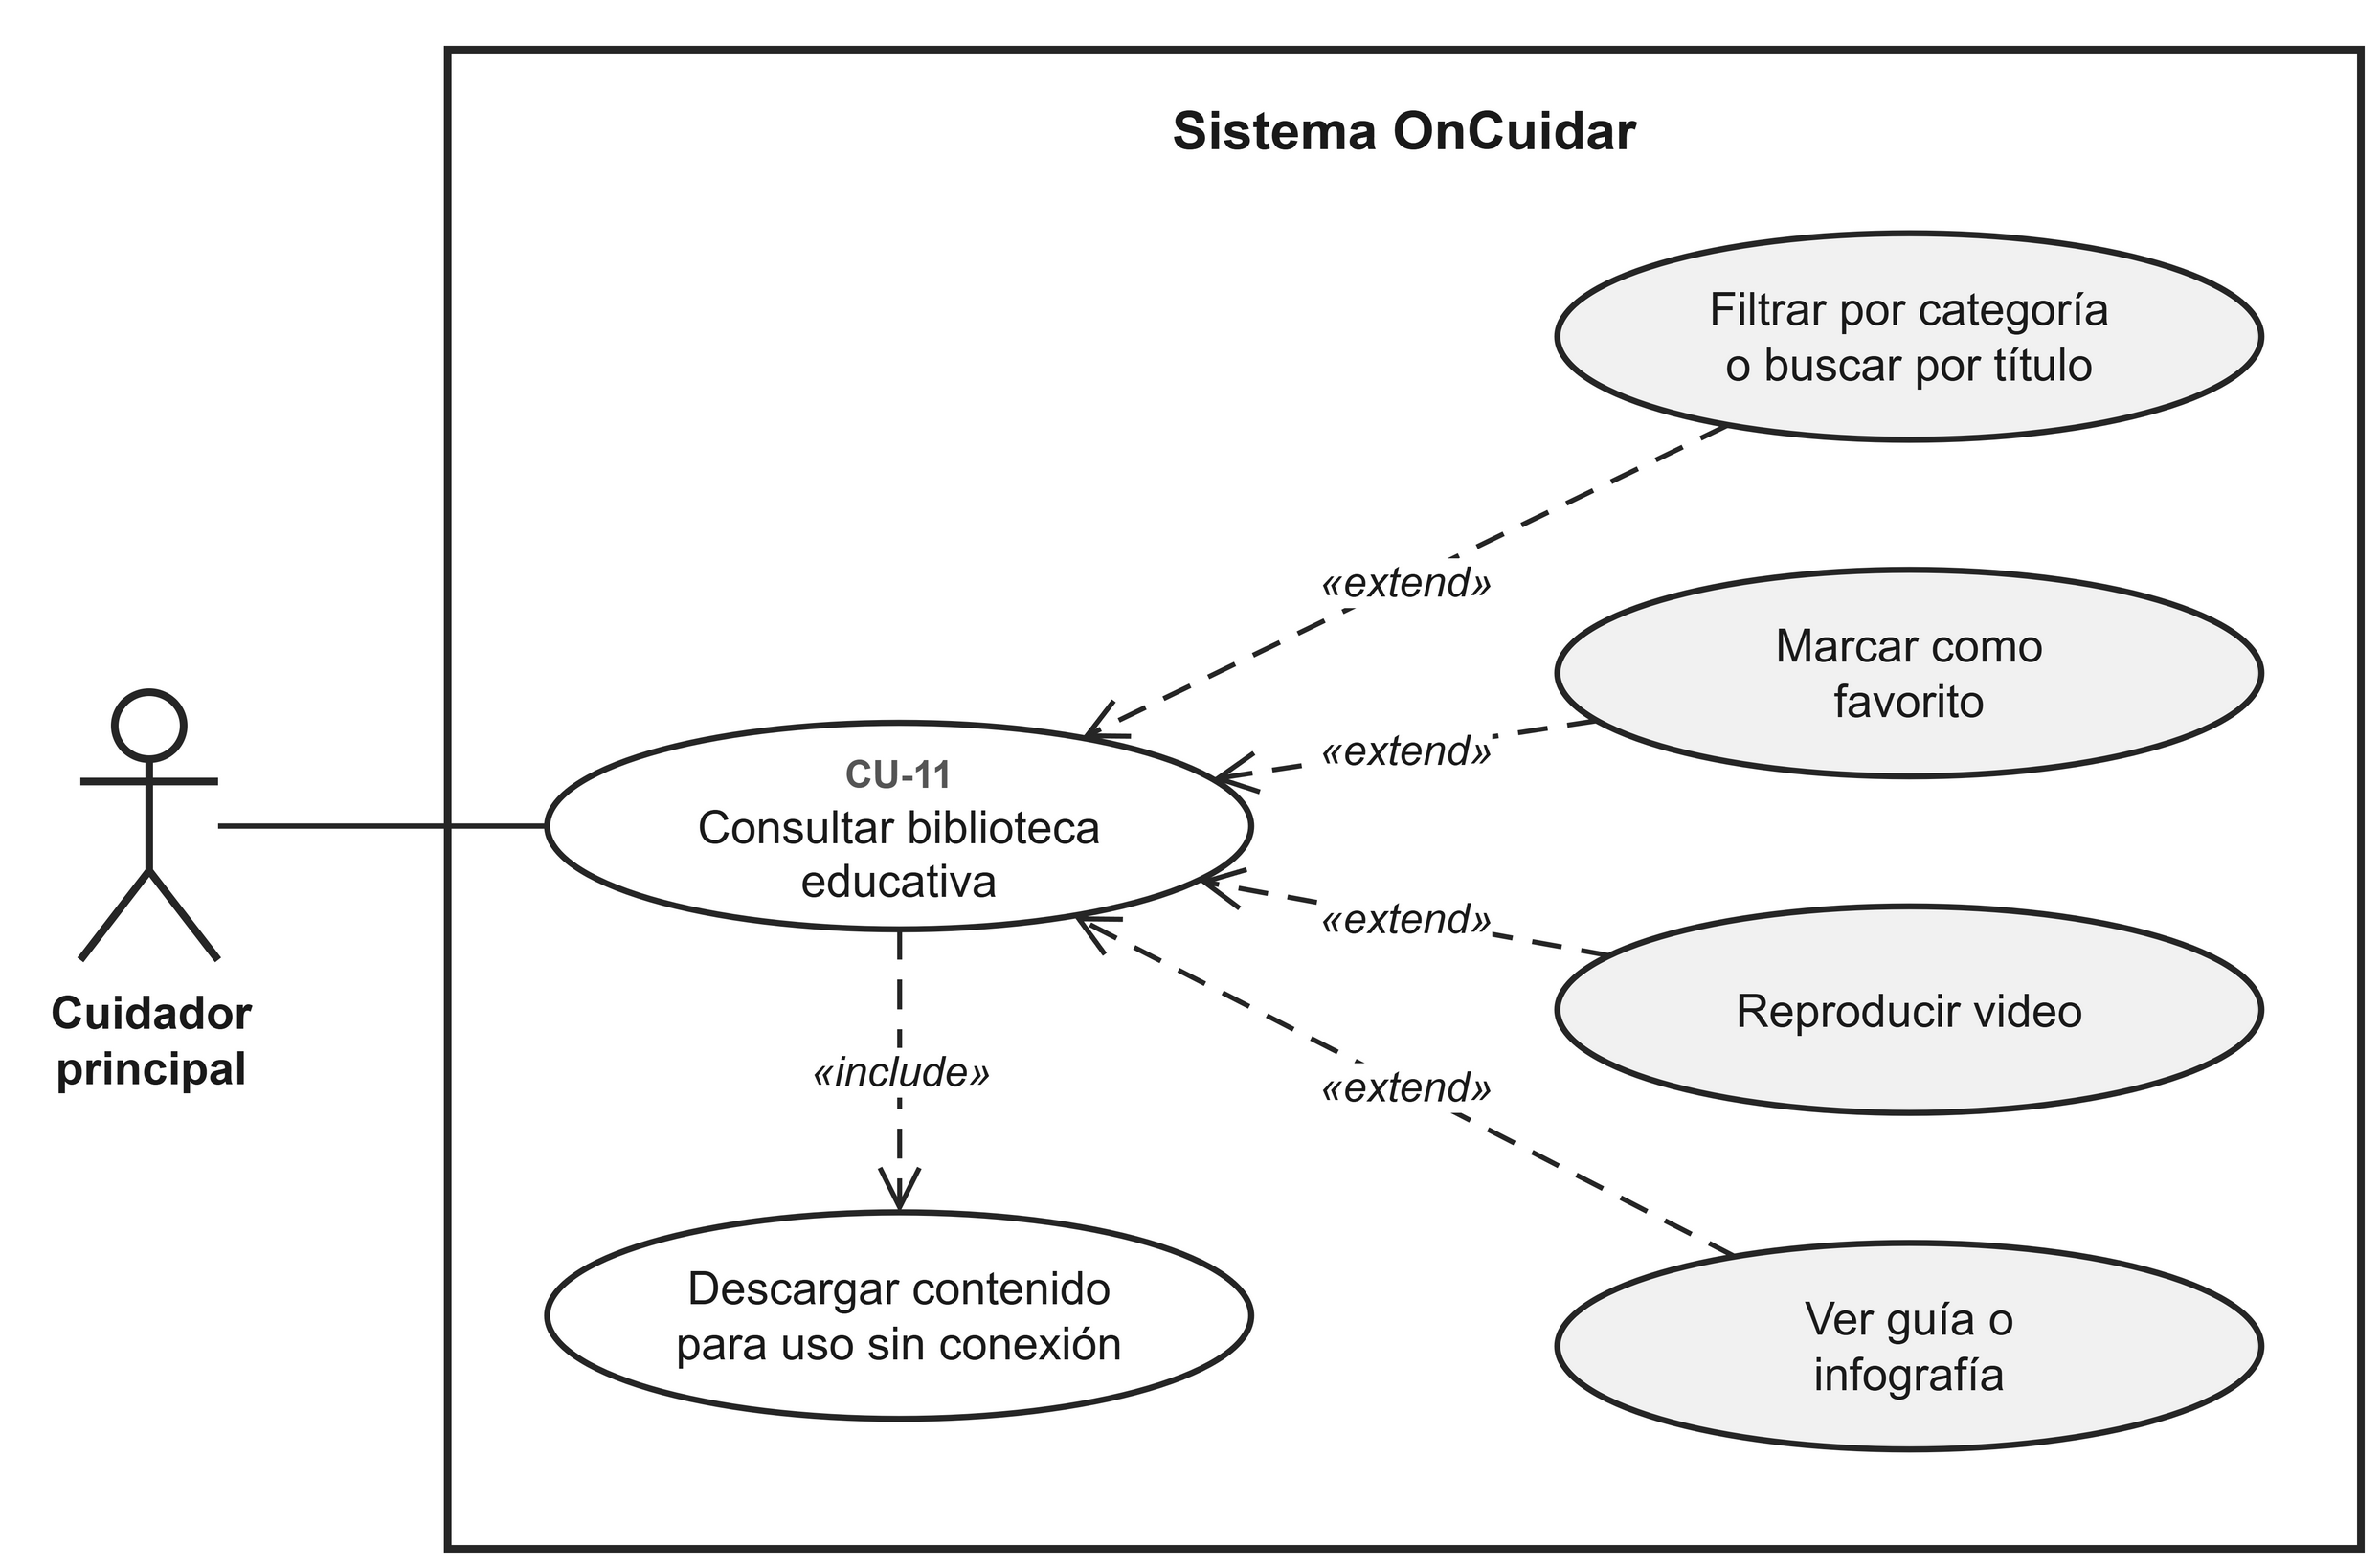
\includegraphics[width=0.9\textwidth, keepaspectratio]{figures/casos-uso/cu-11-biblioteca.png}
    \caption{Diagrama del caso de uso CU-11: consultar biblioteca educativa.}
    \label{fig:cu-11}
\end{figure}

\begin{table}[H]
\centering
\caption{Especificación del caso de uso CU-11.}
\label{tab:cu-11}
\begin{especificacioncu}{CU-11}{Consultar biblioteca educativa}
    \cufila{Descripción}{El cuidador consulta videos, guías, infografías y
    documentos validados por Enfermería, incluso sin conexión.}
    \cufila{Actor}{Cuidador principal.}
    \cufila{Requerimientos}{RF-24, RF-25, RF-26, RF-27.}
    \cufila{Precondiciones}{El cuidador inició sesión y el contenido educativo
    está publicado.}
    \cuflujo{Flujo de eventos básico}
    \cupaso{1. Selecciona Aprende en la barra inferior.}
           {2. Muestra el catálogo con la categoría, el tipo y el estado de
           descarga de cada material.}
    \cupaso{3. Filtra por categoría o busca por título.}
           {4. Muestra los materiales que coinciden.}
    \cupaso{5. Abre un material.}
           {6. Presenta el material según su tipo: reproduce el video, muestra la
           guía o amplía la infografía.}
    \cupaso{7. Marca el material como favorito.}
           {8. Guarda el favorito en la cuenta del cuidador.}
    \cufinflujo
    \cuflujo{Flujos alternativos}
    \cupaso{}{4a. Si no hay coincidencias, informa que no se encontraron
           materiales.}
    \cupaso{}{6a. Si no hay conexión, abre el material desde la copia
           descargada en el dispositivo.}
    \cufinflujo
    \cufila{Postcondiciones}{Los favoritos quedan guardados en la cuenta del
    cuidador.}
\end{especificacioncu}
\end{table}

\subsubsection{Caso de uso: Gestionar recordatorios}

\begin{figure}[H]
    \centering
    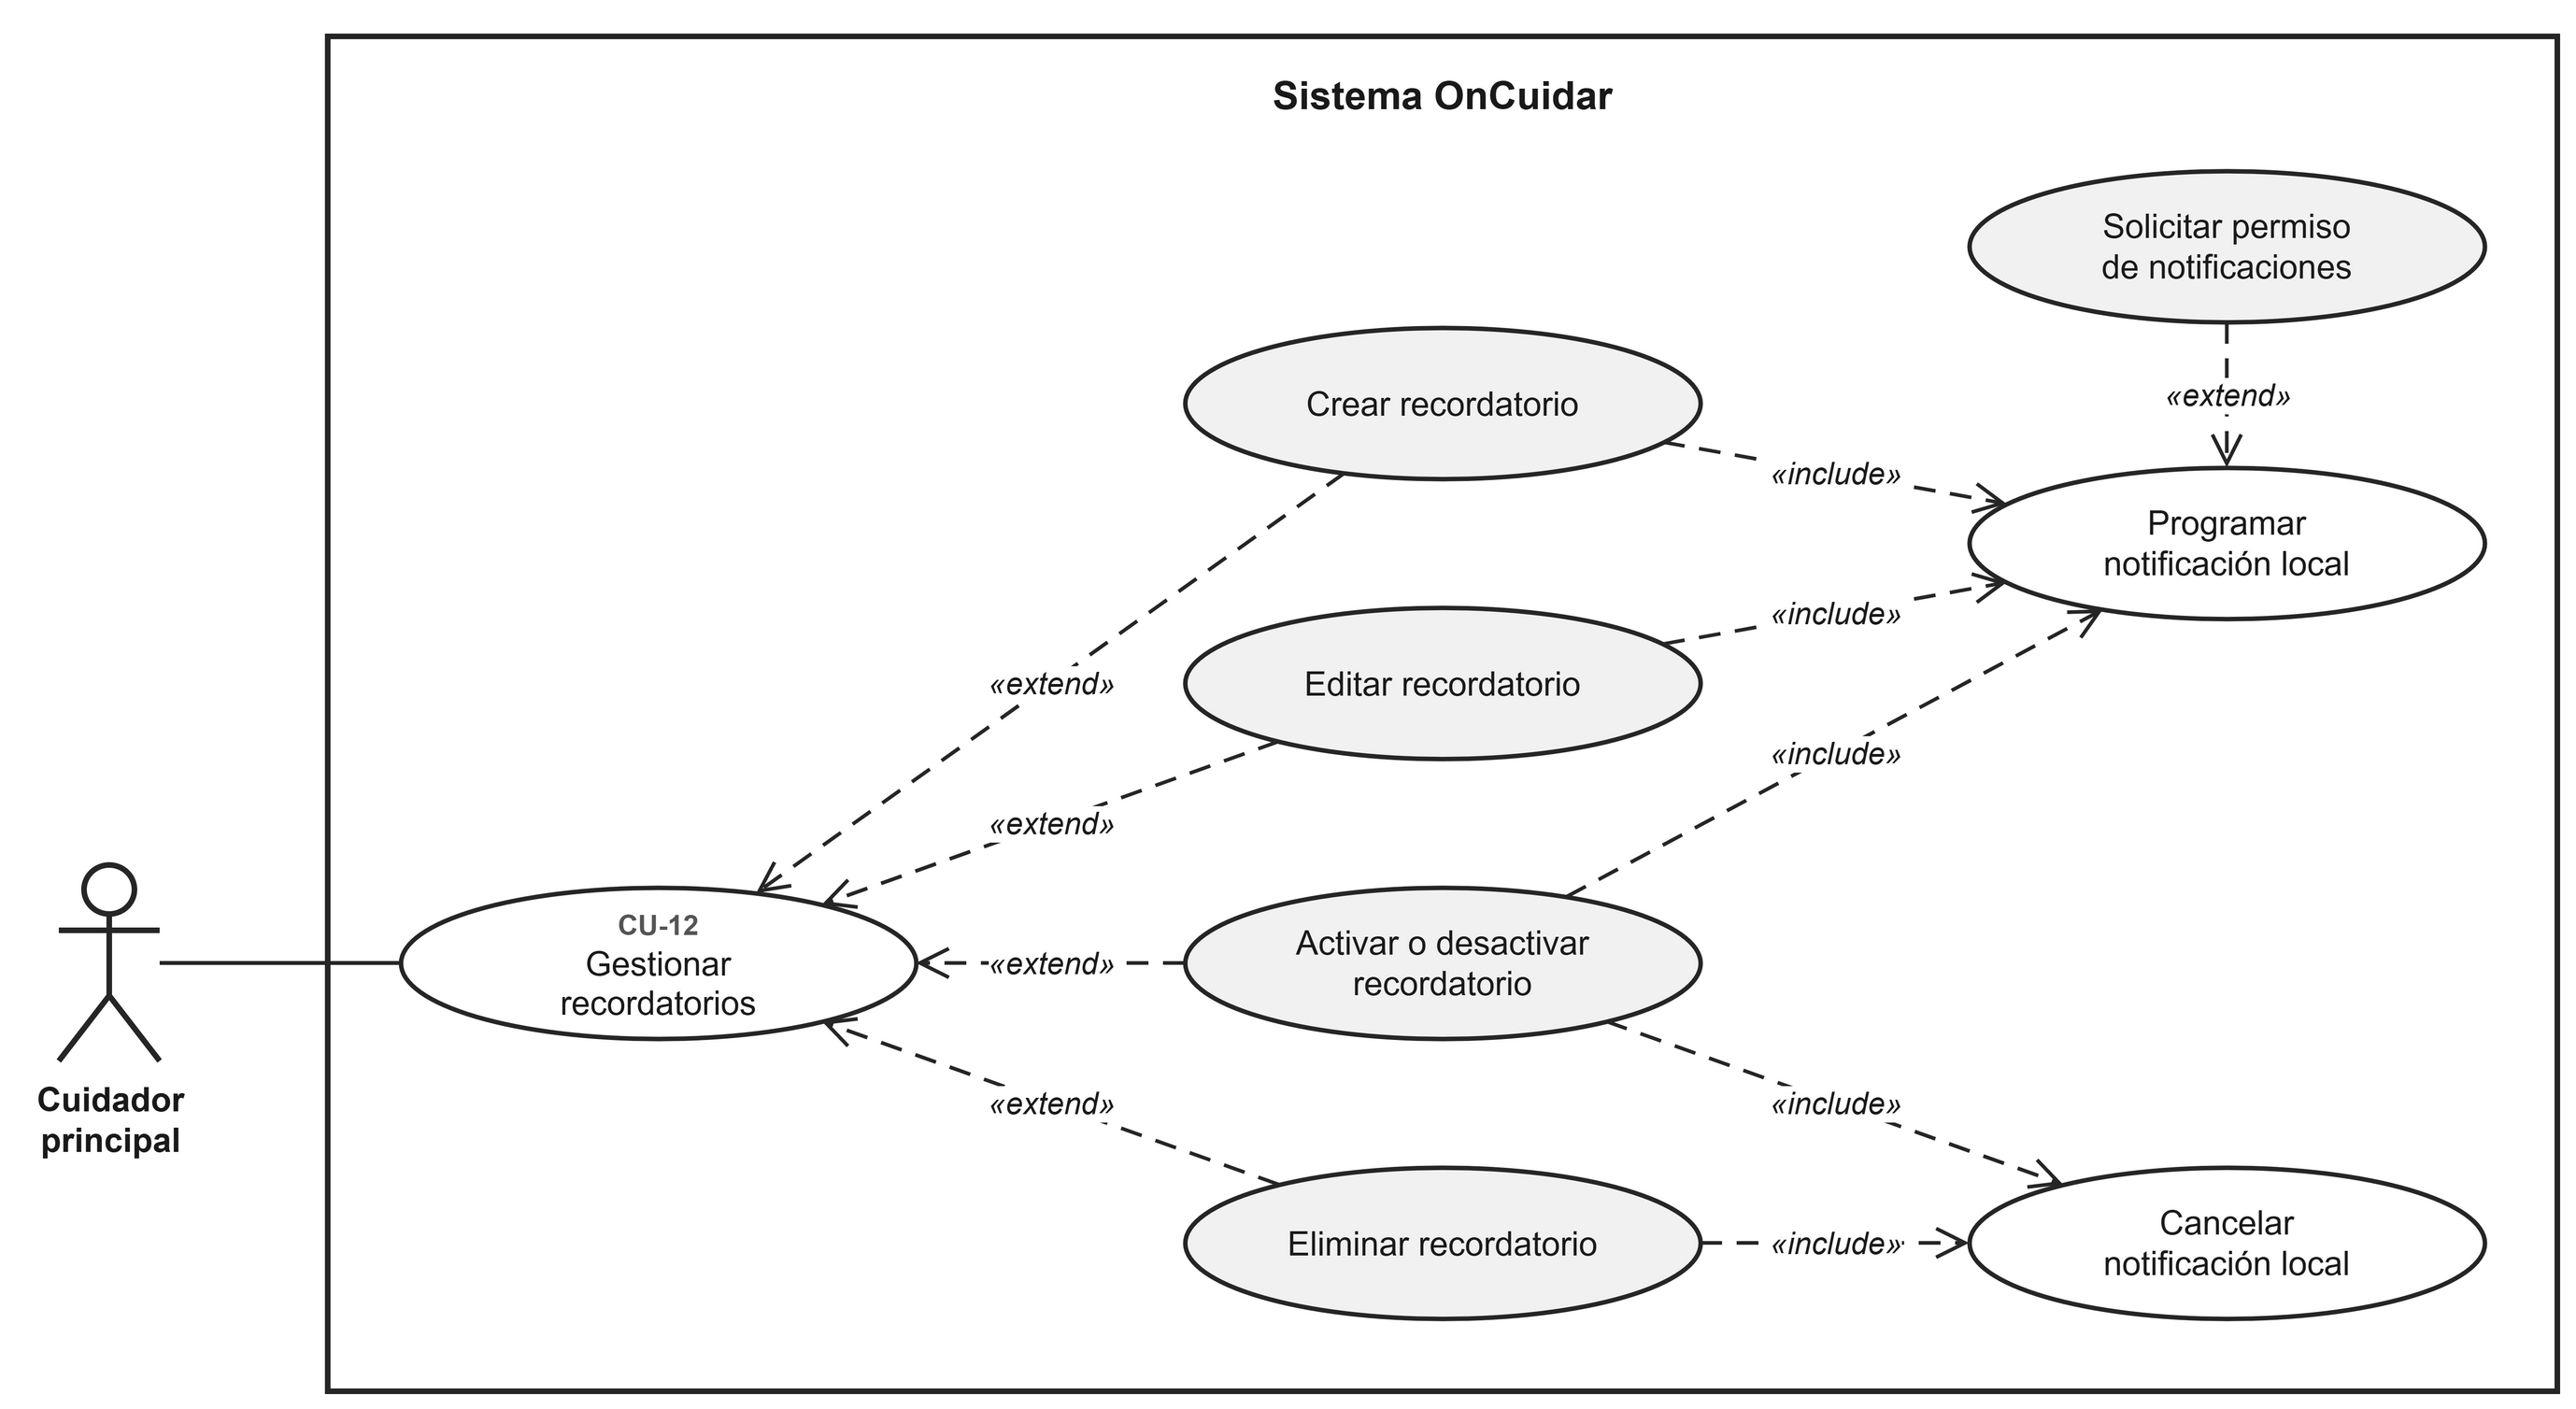
\includegraphics[width=0.9\textwidth, keepaspectratio]{figures/casos-uso/cu-12-recordatorios.png}
    \caption{Diagrama del caso de uso CU-12: gestionar recordatorios.}
    \label{fig:cu-12}
\end{figure}

\begin{table}[H]
\centering
\caption{Especificación del caso de uso CU-12.}
\label{tab:cu-12}
\begin{especificacioncu}{CU-12}{Gestionar recordatorios}
    \cufila{Descripción}{El cuidador programa recordatorios de medicamentos,
    mediciones, citas u otras tareas del paciente activo y recibe una
    notificación a la hora indicada.}
    \cufila{Actor}{Cuidador principal.}
    \cufila{Requerimientos}{RF-22, RF-23.}
    \cufila{Precondiciones}{El cuidador inició sesión y tiene un paciente
    activo.}
    \cuflujo{Flujo de eventos básico}
    \cupaso{1. Abre Recordatorios desde el panel principal.}
           {2. Lista los recordatorios del paciente activo.}
    \cupaso{3. Crea un recordatorio con título, descripción, tipo, fecha, hora
           y repetición.}
           {4. Valida los datos, guarda el recordatorio y programa la
           notificación local.}
    \cupaso{}{5. A la hora programada, muestra la notificación en el
           dispositivo.}
    \cupaso{6. Desactiva o reactiva un recordatorio con su interruptor.}
           {7. Cancela su notificación al desactivarlo o la vuelve a programar al
           reactivarlo, sin borrar el recordatorio.}
    \cufinflujo
    \cuflujo{Flujos alternativos}
    \cupaso{3a. Edita un recordatorio existente.}
           {3b. Guarda los cambios y reprograma la notificación.}
    \cupaso{3c. Elimina un recordatorio.}
           {3d. Pide confirmación y cancela la notificación programada.}
    \cupaso{}{4a. Si es el primer recordatorio, solicita el permiso de
           notificaciones del dispositivo.}
    \cufinflujo
    \cufila{Postcondiciones}{El recordatorio queda guardado y su notificación
    programada en el dispositivo.}
\end{especificacioncu}
\end{table}

\section[Modelamiento de Datos]{Modelamiento de datos}

El modelo de datos representa la información que gestiona OnCuidar. El cuidador
atiende a uno o más pacientes, inicia conversaciones con el asistente y marca
material educativo como favorito. Es también quien programa los
recordatorios: el paciente no usa la aplicación ni opera ese módulo. Cada
paciente posee registros clínicos, y cada registro clínico incluye síntomas del
catálogo ESAS, y la intensidad y la nota de cada síntoma son
atributos de esa relación. El mensaje es una entidad débil, porque solo existe
dentro de su conversación y se identifica por su orden en ella. La
Tabla~\ref{tab:entidades-mer} resume las entidades y la
Figura~\ref{fig:modelo-datos} presenta el modelo entidad-relación en notación de
Chen, con la cardinalidad de cada relación indicada como 1, N o M. Los signos
vitales son un atributo compuesto, el nivel de alerta es un atributo derivado,
porque lo calcula el motor de reglas clínicas, y los días de repetición de un
recordatorio son multivaluados. Los atributos completos de cada entidad se detallan en el anexo de
diccionario de datos.

\begin{table}[H]
\centering
\small
\tablazebra
\caption{Entidades y relaciones del modelo de datos.}
\label{tab:entidades-mer}
\begin{tabularx}{\textwidth}{P{0.95}P{1.45}P{1.00}P{0.60}}
\toprule
\filaencabezado \encab{Entidad} & \encab{Propósito} & \encab{Relación} & \encab{Cardinalidad} \\
\midrule
Cuidador & Usuario responsable del seguimiento. & Atiende a Paciente & 1:N \\
Paciente & Niño, niña o adolescente en seguimiento, con su centro de salud y contacto de emergencia. & Posee Registro clínico & 1:N \\
Registro clínico & Valoración fechada con signos vitales y nivel de alerta. & Incluye Síntoma & N:M \\
Síntoma & Catálogo de síntomas de la escala ESAS. & Incluido en Registro clínico & N:M \\
Recordatorio & Aviso que el cuidador programa sobre un paciente, dirigido al paciente o al propio cuidador. & Cuidador programa Recordatorio & 1:N \\
Conversación & Consulta al asistente con su título. & Contiene Mensaje & 1:N \\
Mensaje & Entidad débil con cada pregunta o respuesta. & Pertenece a Conversación & N:1 \\
Material educativo & Contenido de la biblioteca validado por Enfermería. & Cuidador marca como favorito Material educativo & N:M \\
\bottomrule
\end{tabularx}
\end{table}

\newgeometry{left=2cm, right=2cm, top=0.8cm, bottom=0.8cm}
\begin{landscape}
\begin{figure}[p]
    \centering
    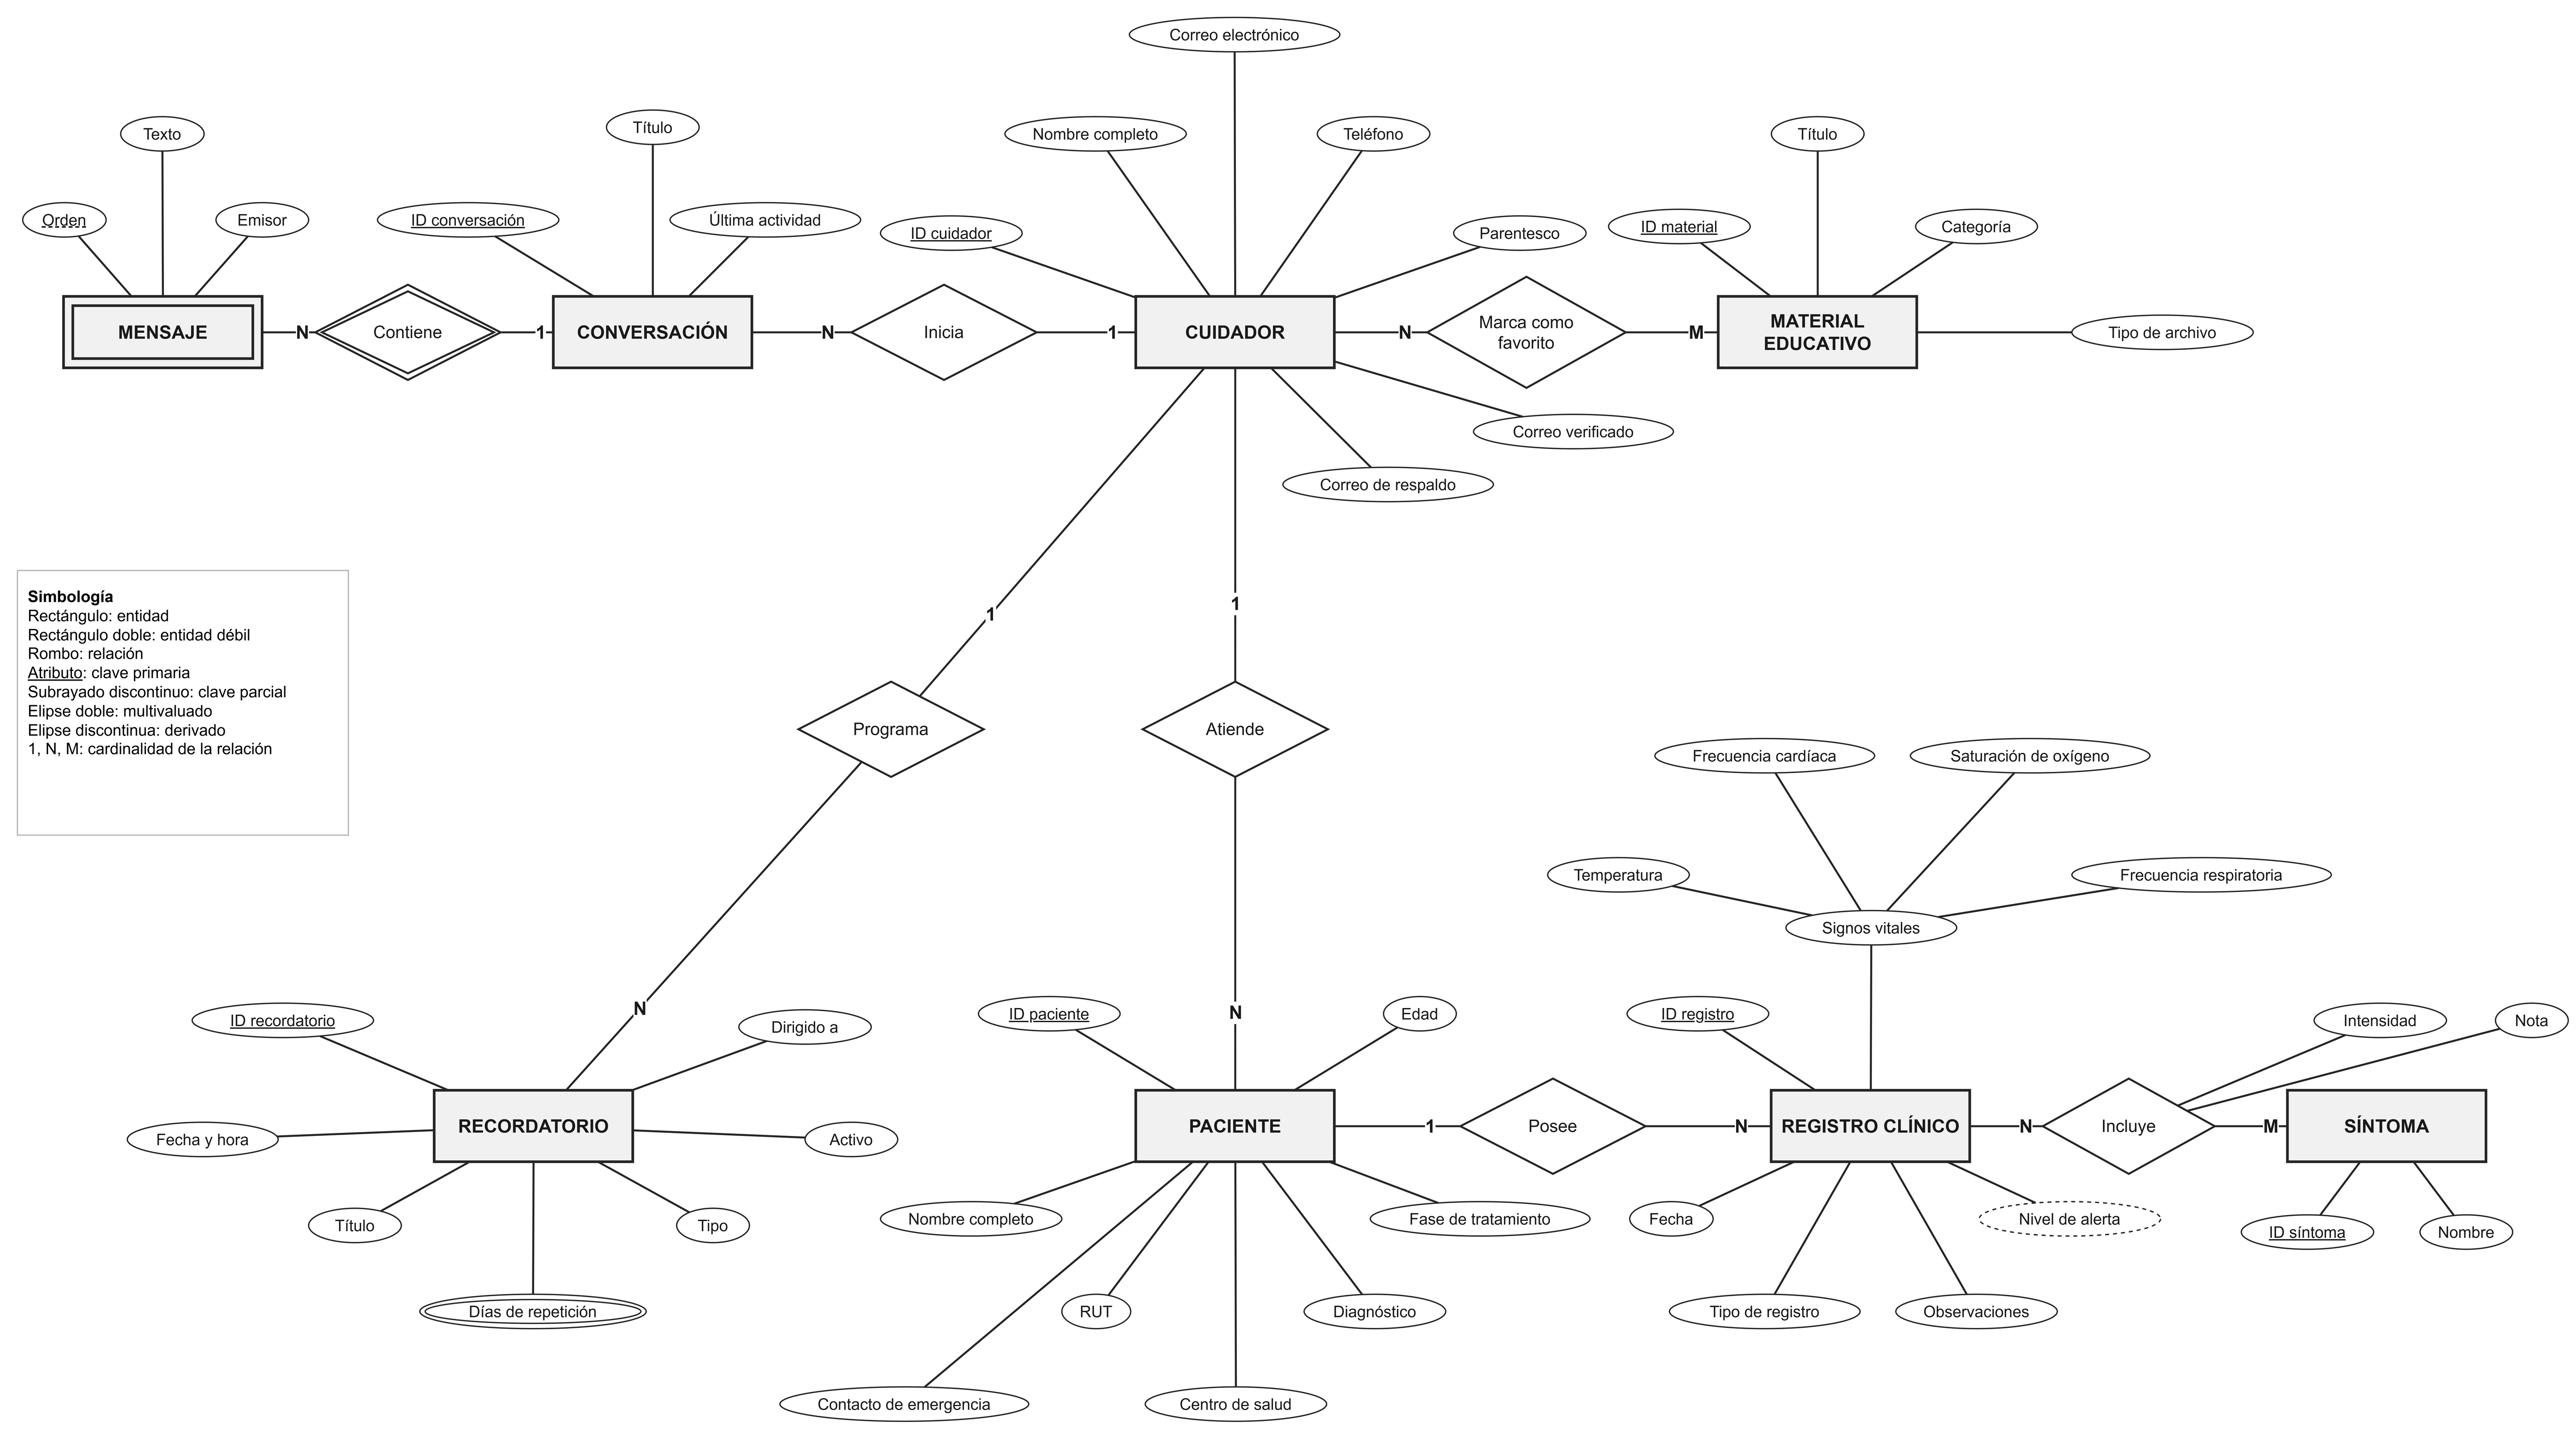
\includegraphics[width=\linewidth, height=0.93\textheight, keepaspectratio]{figures/mer/mer.png}
    \caption{Modelo entidad-relación de OnCuidar.}
    \label{fig:modelo-datos}
\end{figure}
\end{landscape}
\restoregeometry

Al pasar al modelo físico, cada entidad del modelo conceptual se transforma en
una tabla relacional de PostgreSQL (Tabla~\ref{tab:paso-fisico}). El cuidador
corresponde a la tabla usuarios y su identificador es la clave primaria. Las
tablas pacientes, conversaciones y favoritos llevan una clave foránea
a usuarios, y registros\_clinicos y recordatorios dependen del
paciente mediante una clave foránea compuesta (usuario y paciente), de modo que
todos los datos de una cuenta se eliminan en cascada al borrarla. La relación
N:M entre el cuidador y el material educativo se resuelve con la tabla puente
favoritos, de clave primaria compuesta, mientras que el catálogo
material\_educativo es compartido y no pertenece a ningún usuario.

El servidor no puede leer los datos clínicos, porque el dispositivo los cifra
antes de enviarlos. Por eso cada tabla combina columnas en claro, que el
servidor necesita para ordenar, filtrar y relacionar (fechas, nivel de alerta,
tipo de registro, estado activo o archivado), con una columna cifrados de
tipo jsonb que contiene el resto de los atributos como texto cifrado. El
modelo conceptual conserva las entidades Síntoma y Mensaje porque expresan el
dominio del problema, pero no se convierten en tablas propias: la intensidad y
la nota de cada síntoma viven dentro del contenido cifrado del registro clínico,
el catálogo ESAS se incluye en la propia aplicación, y los mensajes forman parte
del contenido cifrado de su conversación, ordenados por su posición. Del mismo
modo, el atributo compuesto de signos vitales y los días de repetición de un
recordatorio se almacenan dentro del jsonb cifrado. Además, el diseño físico
incorpora cuatro tablas de apoyo que no corresponden a entidades del dominio:
claves\_datos, tokens\_restablecer, tokens\_correo y
esperas\_recuperacion, que resuelven la seguridad de la cuenta. El
Anexo~E detalla todas las columnas.

\begin{table}[H]
\centering
\small
\tablazebra
\caption{Transformación del modelo conceptual a tablas relacionales.}
\label{tab:paso-fisico}
\begin{tabularx}{\textwidth}{P{0.90}P{1.00}P{1.10}}
\toprule
\filaencabezado \encab{Elemento conceptual} & \encab{Tabla o estructura física} & \encab{Clave y relación} \\
\midrule
Cuidador & usuarios & Clave primaria uuid; correo único. \\
Paciente & pacientes & Clave primaria (usuario, paciente); clave foránea a usuarios. \\
Registro clínico & registros\_clinicos & Clave primaria (usuario, paciente, registro); clave foránea compuesta a pacientes. \\
Recordatorio & recordatorios & Misma clave compuesta; el paciente al que se dirige es la clave foránea. \\
Conversación y Mensaje & conversaciones & Clave primaria (usuario, conversación); los mensajes van en el jsonb cifrado. \\
Material educativo & material\_educativo & Clave primaria de texto; catálogo compartido. \\
Marca como favorito (N:M) & favoritos & Tabla puente con clave primaria (usuario, material). \\
Síntoma e Incluye (N:M) & Contenido cifrado del registro & Catálogo en la aplicación; sin tabla propia. \\
\bottomrule
\end{tabularx}
\end{table}
